
\chapter{Experimentation-TODO}
\label{ch:Experimentation}

This chapter covers the experiment design and setup, describing in detail results obtained during different phases and tests. This chapter is organized as follows: first, we discuss the results of the training and its validation in Section~\ref{sec:TrainingResults}, then in Section~\ref{sec:AutoencoderResults} and Section~\ref{sec:GeneratorResults} we explore the DL model performance from the perspective of each component individually using the methods defined in Section~\ref{sec:EvaluationMethods}.  Lastly, in Section~\ref{sec:ModelPerformance}, we analyze the performance of the DL model based on the two main evaluation metrics defined in Section~\ref{sec:ResearchObjectiveandSolution} (MSE and execution time).

Results from experiments in this chapter are based on the dataset described in Section~\ref{sec:DataCollection}. The experiments performed can be categorized into two main types based on the obstacle shape used:
\begin{enumerate}
    \item Circular obstacle: the obstacle is randomly positioned in the simulation space, and its size is given by radius $\textbf{r} = qH$, where $q \in [\frac{1}{9}, \frac{1}{5}]$ and $H$ is the height of the simulated region.
    
    \item Elliptical obstacle: the obstacle is also randomly positioned in the space, and its size is given by semi-major axis $\textbf{a}=qH$, where $q \in [\frac{1}{5}$, $\frac{1}{3}]$ and $H$ is the simulated region height, and the semi-minor axis $\textbf{b}=p\textbf{a}$, where $p \in [\frac{1}{5}, \frac{1}{4}]$. The ellipse is also tilted with an angle $\boldsymbol{\alpha} \in [-30^\circ, 30^\circ]$ with respect to $\textbf{a}$ and the Cartesian $x$-axis.
\end{enumerate}

The ranges of the obstacle dimensions and positions were chosen to fully fit the shape inside the simulated space without touching its perimeter. The dimensions of the Ellipse object were chosen to maintain a shape similar to that of an airfoil as described in Section~\ref{sec:DataCollection}, and its inclination range to represent common wing ``angle of attack" including the critical or stalling ``angle of attack" (typically between $18^\circ$ and $25^\circ$ degrees)\cite{abbott_ira_h_summary_1945}.


%----------------------
\section{Training Results}
\label{sec:TrainingResults}
%----------------------

The neural network was trained for 500 epochs, across which, the Mean Squared Error (MSE) loss functions results were collected for both the Autoencoder and the Generator. The training error is captured in  Both plots in Figure~\ref{fig:loss} show that the is generally lower than the validation error; this is to be expected given the proposed model was evaluated with sequences used during the training process. 

\begin{figure}[H]
    \centering
    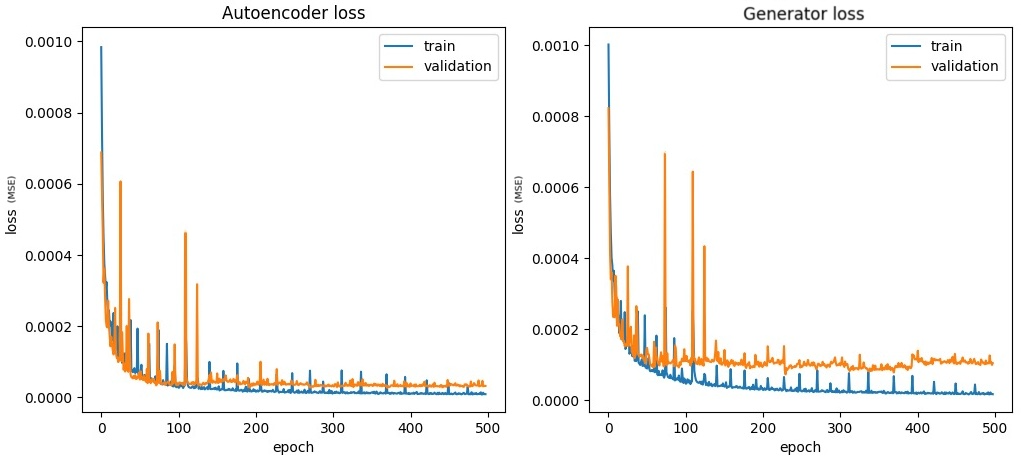
\includegraphics[width=1\linewidth]{images/model_training.png}
    \caption{Autoencoder and Generator loss evolution during training}
    \label{fig:loss}
\end{figure}

Figure \ref{fig:loss} demonstrates the stability of the MSE loss function's evolution during training. The loss trend quickly descends, and after 200 epochs, the error stabilizes and converges to its final value. In addition, note that the slight difference between the training and validation errors signifies that the model does not excessively over-fit the training data. Regular error spikes appear during training, representing instances where the model encountered local maximums before finding a local minimum. This happens when, during parameter optimization, a new combination of the network’s weights is worse than the previous one, but then it improves again. This further underscores the model's reliability. These spikes decrease as the training advances, indicating a stable and reliable training process. Another critical aspect to note is that those spikes happen almost on the same epoch number and with a similar intensity for both of the model's components (Autoencoder and Generator), meaning that these components are working in collaboration to find the best result. This supports the election of the model architecture.

\begin{table}[h]
    \caption{Training and Testing errors (MSE)}
    \centering
    \begin{tabular}{|c|c|c|}
    \hline
             & Autoencoder & Generator \\ \hline
    Training & $7.7727\times10^{-06}$ & $1.5429\times10^{-05}$ \\ \hline
    Validation  & $3.2173\times10^{-05}$ & $2.0414\times10^{-05}$ \\ \hline
    \end{tabular}
    \label{tab:errors}
\end{table}

A comparison between training and validation errors is displayed in Table~\ref{tab:errors} for both the Autoencoder and Generator components of the model. The low error rate in all cases indicates the model's good performance. It is important to remember that validation samples were not used during training, which is noticeable in how lower the training errors are compared to the validation errors. Since the model has already ``seen" the training samples to optimize its weights, it learns how to approximate the output based on those values.

In the following sections, we analyze the model's performance more deeply, examining each component's performance individually.

%----------------------
\section{Autoencoder Results}
\label{sec:AutoencoderResults}
%----------------------

To evaluate the Autoencoder, we need to verify that the Decoder can reconstruct the original information using the low-resolution representation of the data created by the Encoder. Because the input to the model is a set of frames according to the window described in Chapter~\ref{ch:Methods}, the Decoder output will also have those dimensions. This means that to evaluate the Decoder's output, we must compare all the frames in the set. 

Using the Decoder's output sequence representing the fluid state, a \textit{heatmap} of fluid velocity values was rendered to compare the results visually. Figure~\ref{fig:ReconstructedFrames} shows examples of frames with each type of obstacle. In each case, we show the Original frame to the left and the Reconstructed frame output by the Decoder to the right. We can see that although there are some minor differences, both frames are almost identical. Similar results were obtained for the rest of the sequences. The differences found can be seen in small changes of intensity of the \textit{heatmap} colors, which may indicate that the velocity values approximate the original ones but are either lower or higher than expected. Although there are some minor differences, the similarities between the Original and Reconstructed frames give us a clue that the Autoencoder is working as intended.

\begin{figure}[!htbp]
    \centering
    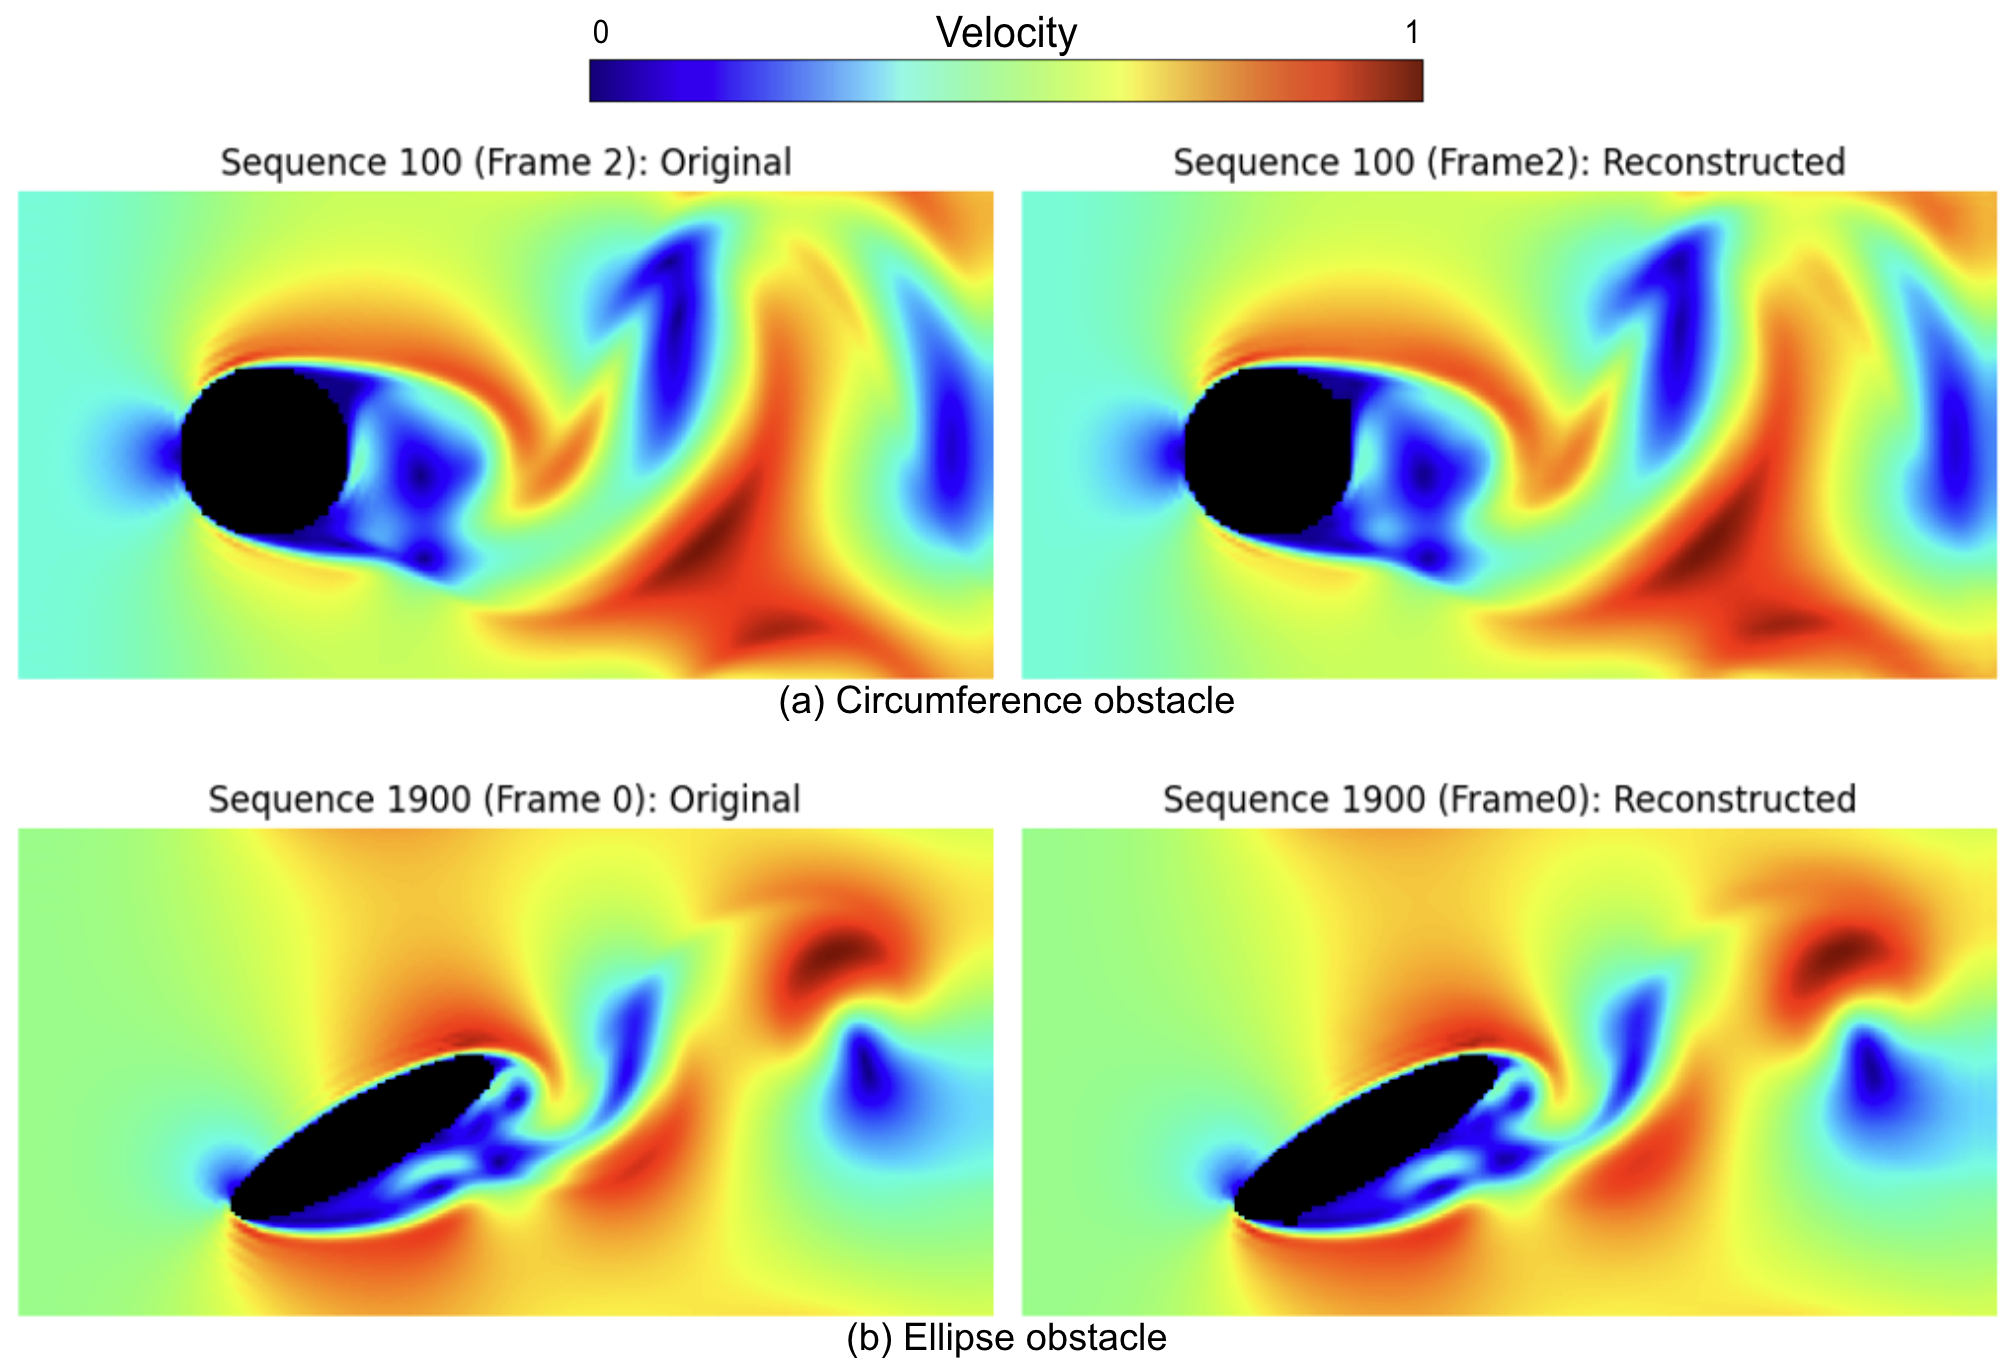
\includegraphics[width=1\linewidth]{images/autoencoder_frames.png}
    \caption{Original vs Reconstructed frames}
    \label{fig:ReconstructedFrames}
\end{figure}

For the following evaluation method, we compare the velocity values between the Original and Reconstructed frames to verify their similarity. This is done by creating a histogram of velocities, i.e., a frequency count of velocity values on each grid cell in the frame. Figure~\ref{fig:ReconstructedHistograms} shows examples of those histograms for Origianl and Reconstructed frames containing each type of obstacle. The frame examples are the same as Figure~\ref{fig:ReconstructedFrames} used in the previous evaluation method. On the x-axis, we have the range of all the velocity values in the frame. These values are between 0 and 1 because the data was previously normalized, as explained in Section~\ref{sec:DataPreparation}. On the y-axis, the frequency or occurrence of each velocity value is represented. To compare all the velocity histograms, we calculated the Jensen-Shannon distance between each frequency distribution. The resulting average distance between the original and reconstructed frames was 0.021, with a standard deviation of 0.014.

% In the example shown, we can see a lot of coincidence between the corresponding histogram bars of each frame. Similarly to the previous evaluation, we can see some differences between the histogram bars, but nothing significant. Some of the bars are taller or shorter, coinciding with the color intensity difference observed in the \textit{heatmaps} of the previous evaluation. Similar results were observed on the histograms of other sequences.

\begin{figure}[H]
    \centering
    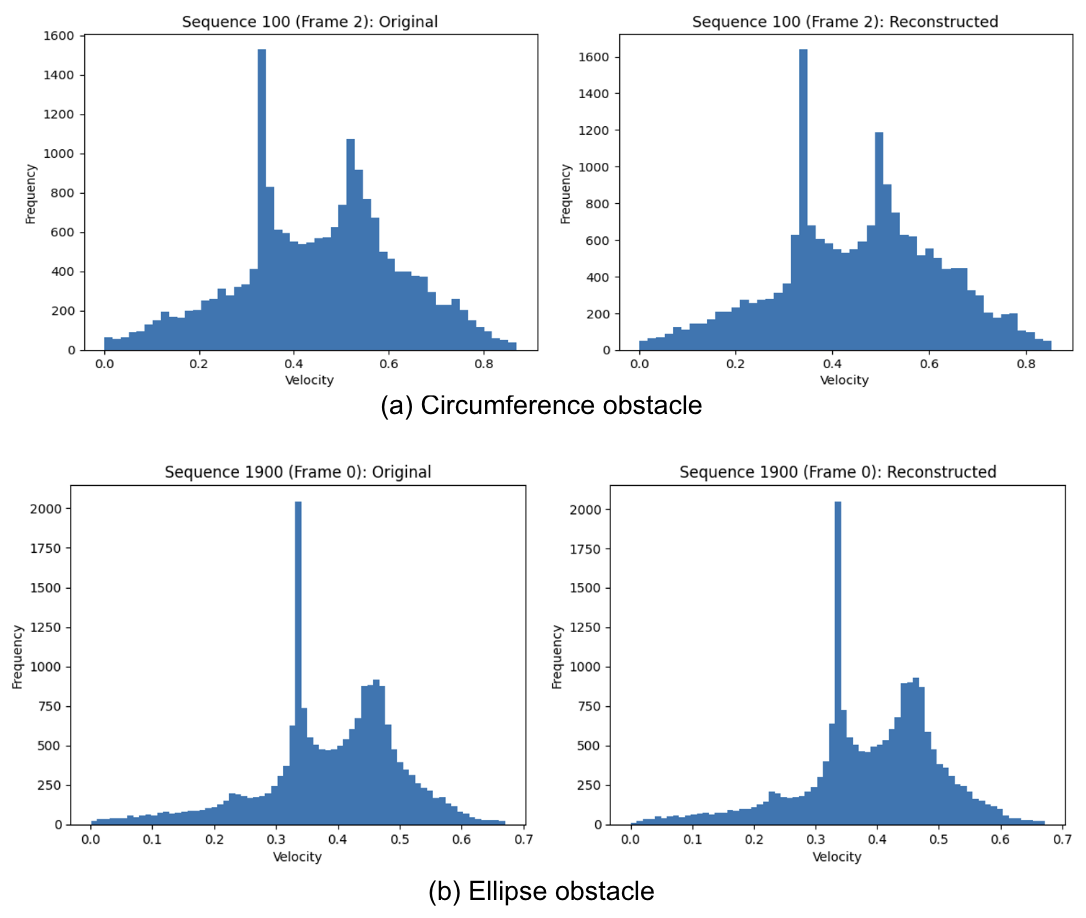
\includegraphics[width=1\linewidth]{images/autoencoder_histogram.png}
    \caption{Original vs Reconstructed frames velocity histograms}
    \label{fig:ReconstructedHistograms}
\end{figure}

Both evaluations tell us that the Autoencoder successfully reduces the data's dimensionality so that the original data can be reconstructed using that low-resolution representation. This means that the training of this model's component was successful. Although there are some minor errors, the fluid flow structure remains correct, and the approximations of the velocities are very close.

The Autoencoder is a vital component of the model because it guarantees that the model successfully extracts enough information to represent the original data. This process of reducing the amount of information with a lower representation is important to support the next phase, which is the generation of the next fluid state.

%----------------------
\section{Generator Results}
\label{sec:GeneratorResults}
%----------------------

The Generator's goal is to generate the next fluid flow state using as an input the low-resolution representation created by the Encoder. To evaluate this component, the resulting frame is compared against the expected frame taken from the dataset created by the numerical simulation. For this evaluation we used similar methods than the Autoencoder evaluation.

Figure~\ref{fig:GeneratedFrames} shows a comparison between a generated frame velocity \textit{heatmap} at the right, and the expected frame at the left. The images show a result example for each of the possible obstacle types. Similar to the Autoencoder results, very small differences appear in the \textit{heatmap} colors, however, both images are almost similar.

We created the velocity histogram for each generated frame and compared it to the original frame. Figure~\ref{fig:GeneratedHistograms} compares 2 examples of the velocity histograms. Then, we calculated the Jensen-Shannon distance between the velocity distributions of the frames in all the sequences. This results in an average distance between the expected and generated frames of 0.043 with a standard deviation of 0.010. The low average value of the distance metric between both distributions indicates that the original and generated frames are very similar.

\begin{figure}[!htbp]
    \centering
    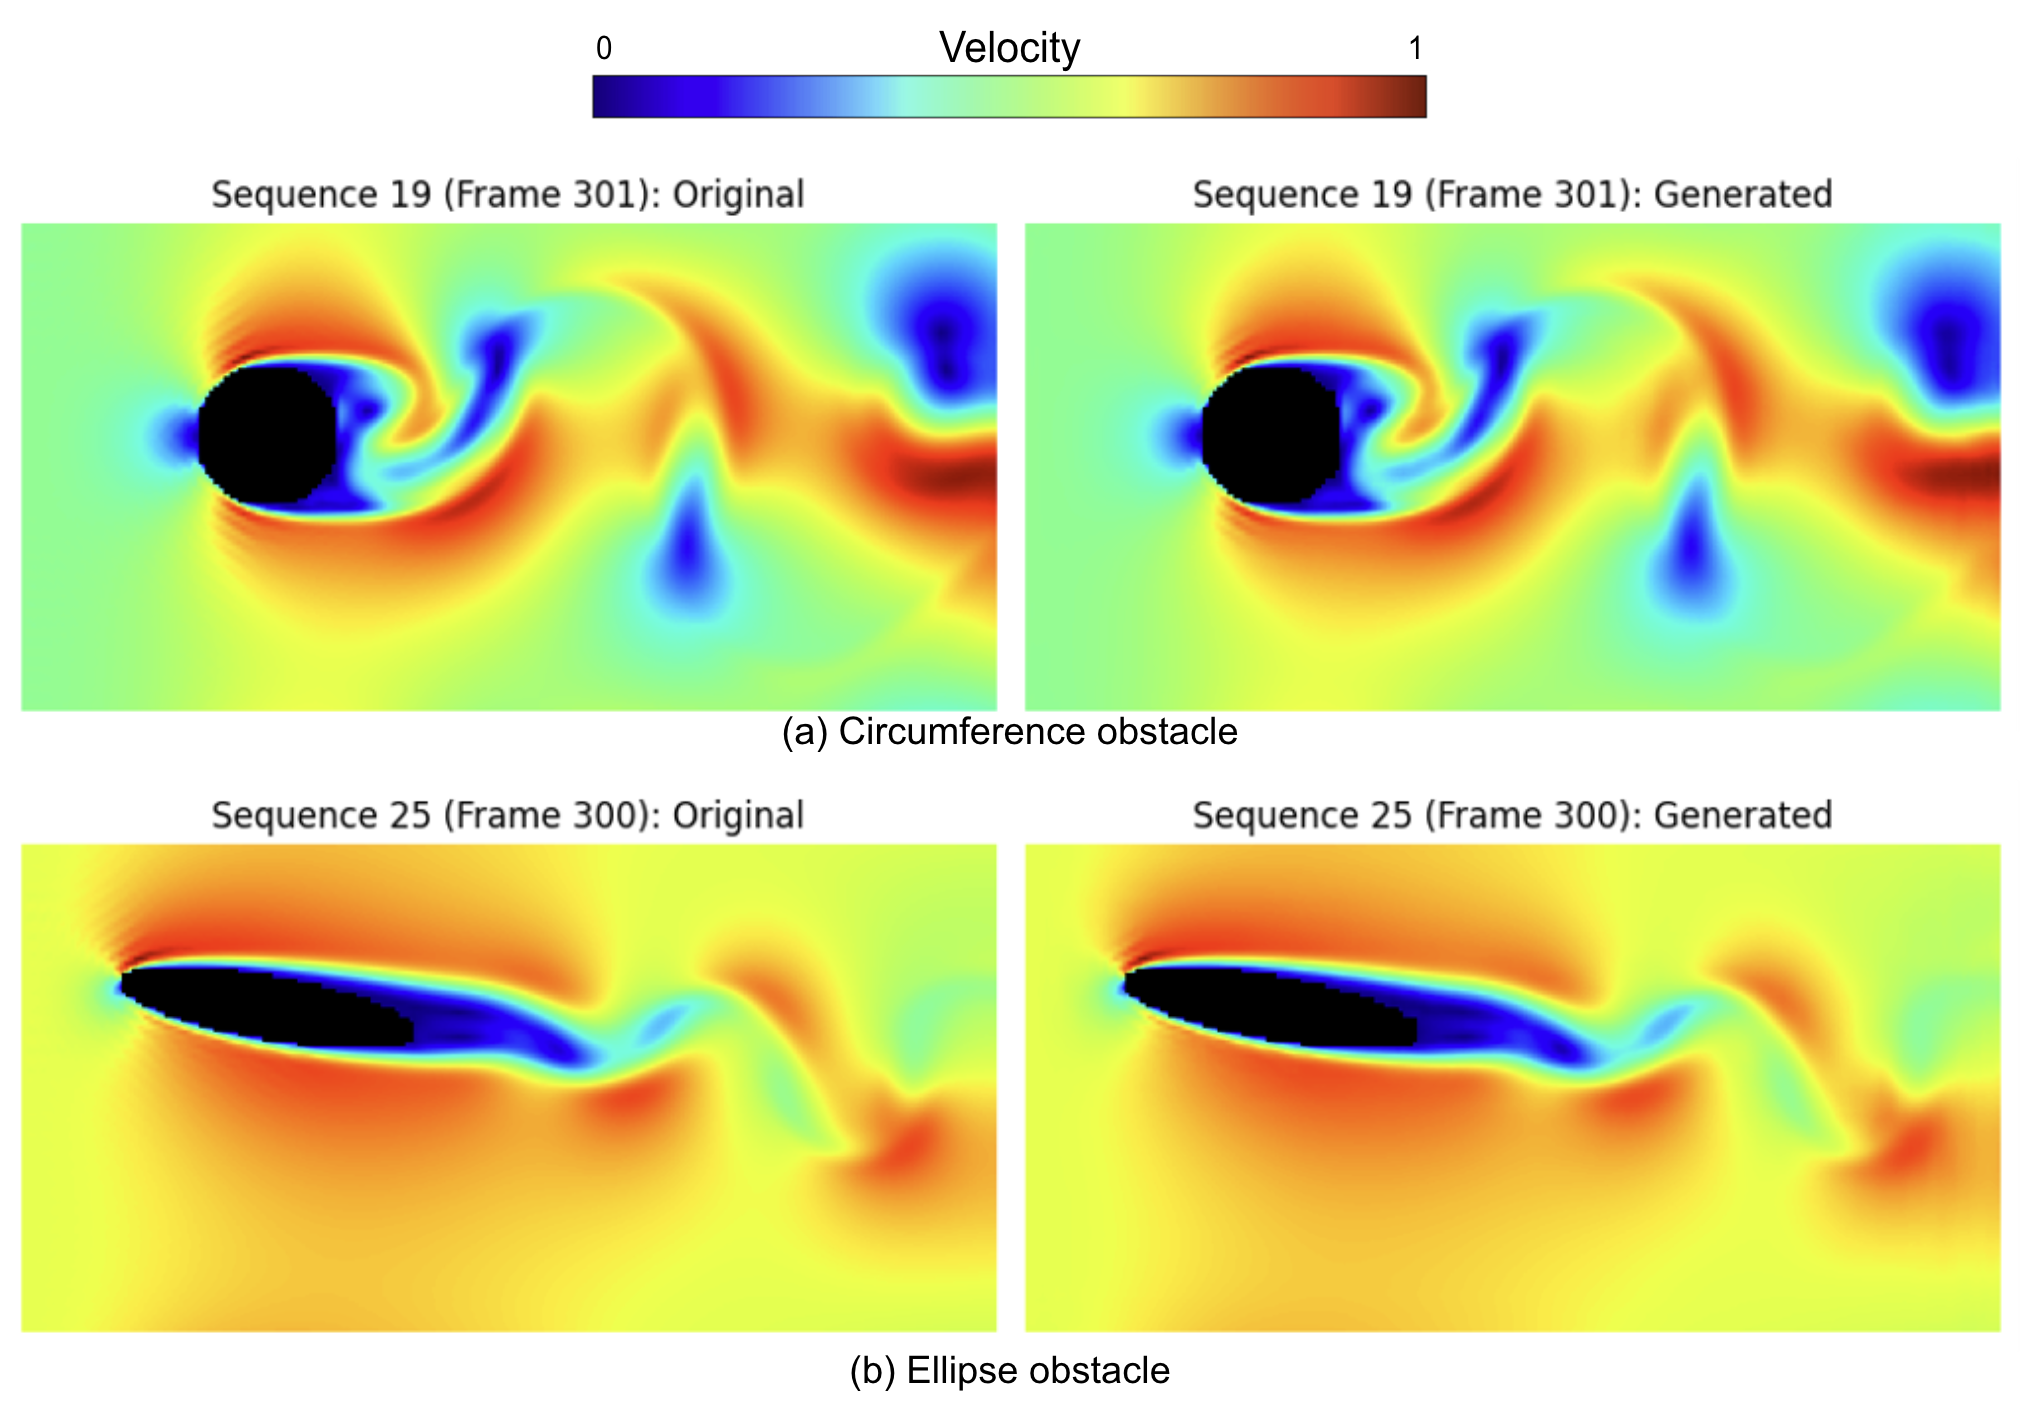
\includegraphics[width=1\linewidth]{images/generator_frames.png}
    \caption{Original vs Generated frames}
    \label{fig:GeneratedFrames}
\end{figure}

\begin{figure}[!htbp]
    \centering
    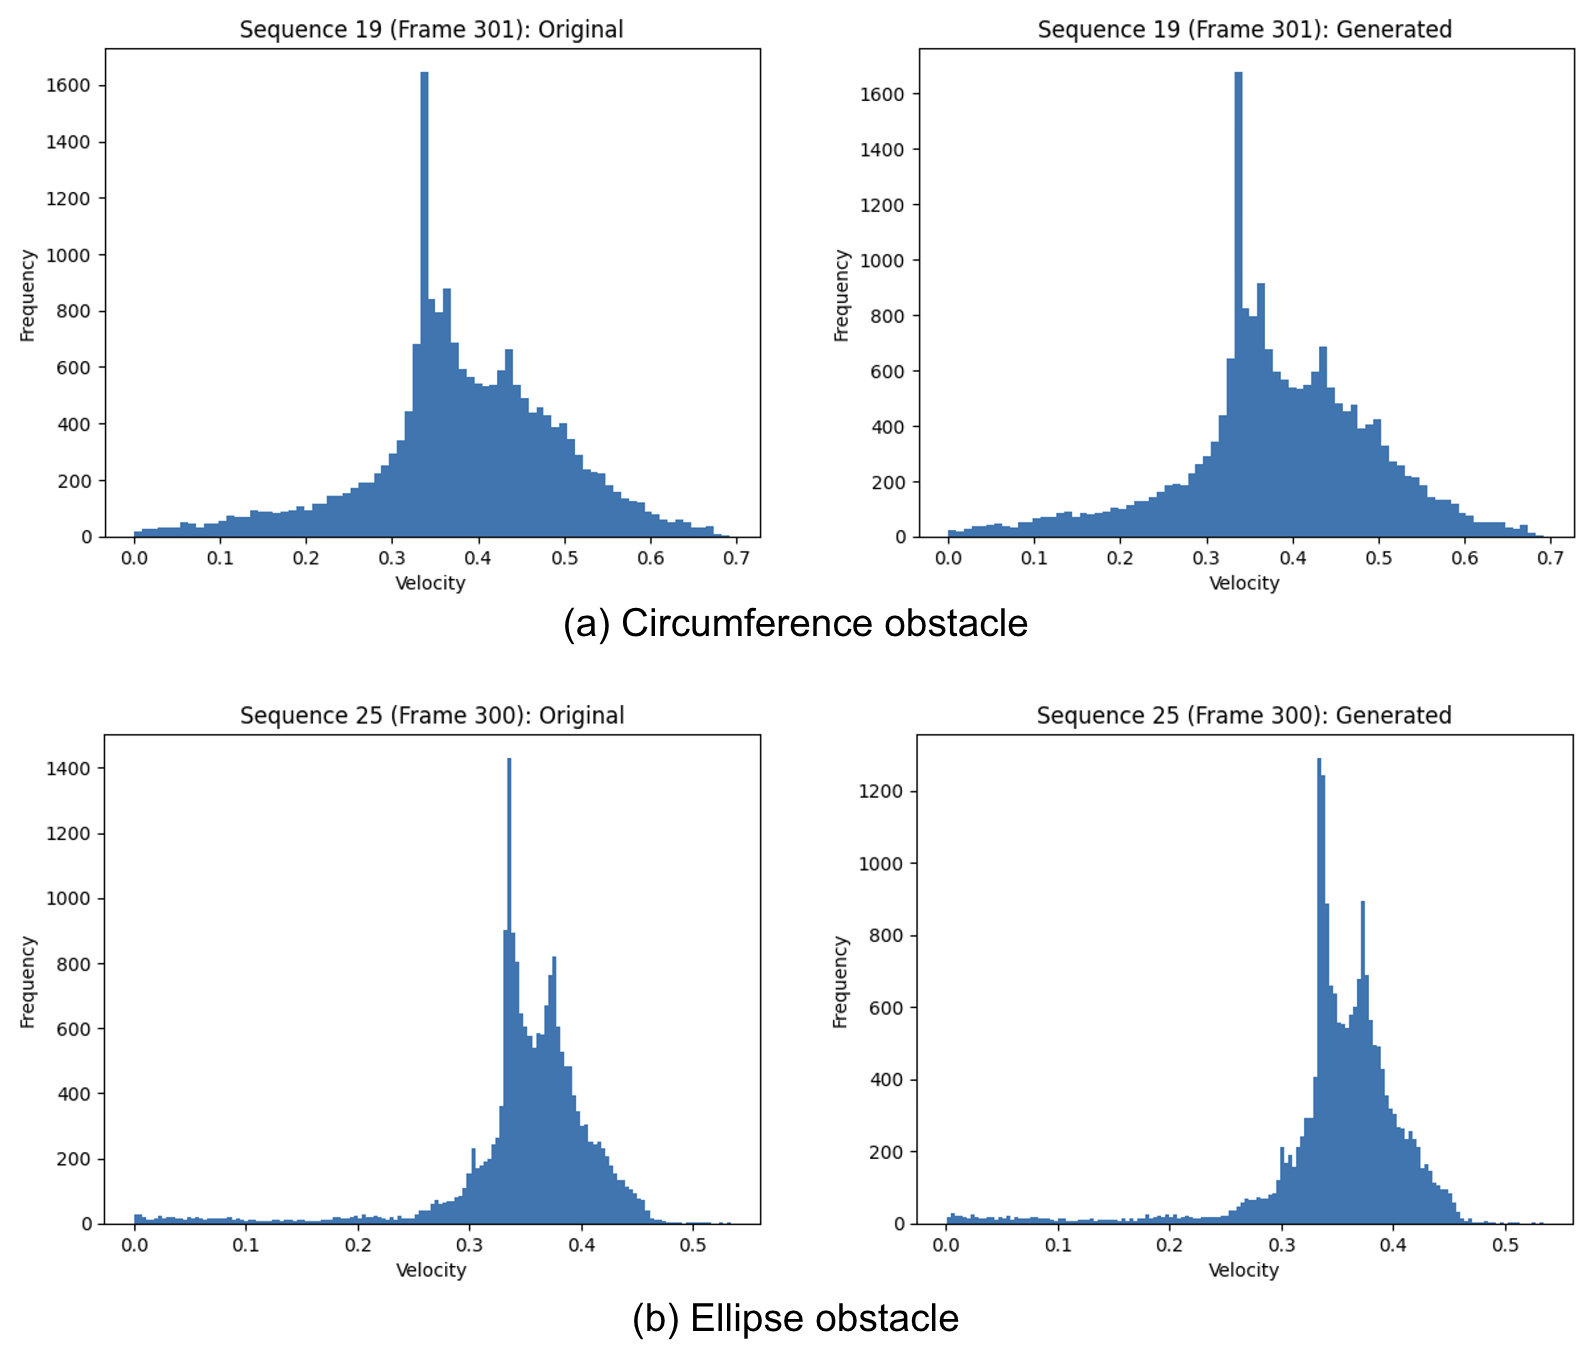
\includegraphics[width=1\linewidth]{images/generated_histogram.png}
    \caption{Original vs Generated frames velocity histograms}
    \label{fig:GeneratedHistograms}
\end{figure}


These evaluations show that the model can successfully approximate the next state in the fluid flow sequence. The same level of accuracy in both evaluation methods was observed across all the cases in the testing dataset. Although there are some differences between the expected and generated frames, the model can replicate the evolution of the fluid flow structure across the sequence simulation time.

%----------------------
\section{Model Performance}
\label{sec:ModelPerformance}
%----------------------

In this section we explore the results of the two main metrics chosen to evaluate this models performance as explained in Section~\ref{sec:ResearchObjectiveandSolution}. These metrics are: the Error measured with MSE, and the execution time of the simulation measured in seconds.

\subsection{Error Measurements}
\label{subsec:ErrorMeasurements}

Figure~\ref{fig:ErrorMeasurements} shows the results of the MSE metric. The results are divided into three groups, one for all the shapes in the dataset together, one with only Circumferences obstacles, and another for Ellipses obstacles. The minimum, maximum, and average error values are plotted for each group. It is important to mention that the dataset is balanced, meaning that the amount of examples with each obstacle type is the same, which is essential to ensure fairness in the results. 

The following analysis can be done by looking at the MSE plots in Figure~\ref{fig:ErrorMeasurements}. We can see that the minimum and maximum errors across the entire dataset are both in simulations with an ellipse obstacle. Additionally, the difference between the minimum and maximum error is lower for the circumference than the ellipse obstacle. This could be caused by circumference obstacles presenting less variability in their shapes, with only a change in the radius, while ellipses obstacles have more diversity in their shapes. This variability in the obstacle shapes makes it more challenging for the model to learn how to simulate the ellipse objects. However, because the average errors are similar between the two types of obstacles, we can conclude that no specific obstacle shape is significantly more difficult for the model to simulate. 

\begin{figure}[!htbp]
    \centering
    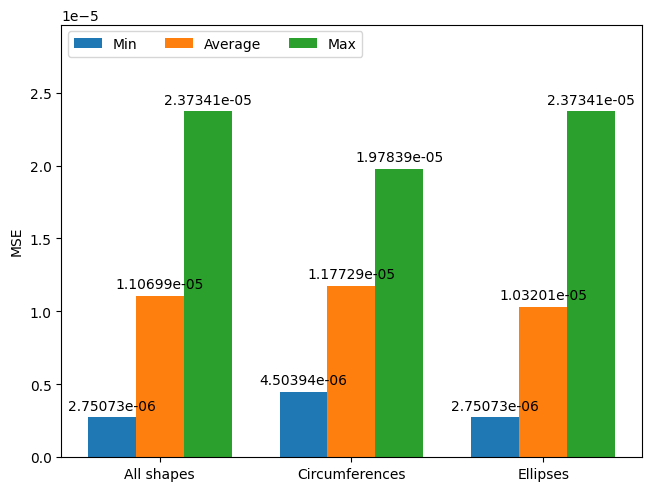
\includegraphics[width=0.7\linewidth]{images/MSE.png}
    \caption{Model MSE error metric}
    \label{fig:ErrorMeasurements}
\end{figure}


\subsection{Execution time}
\label{subsec:ExecutionTime}
As explained in Section~\ref{sec:ResearchObjectiveandSolution}, the goal of this model is to reduce the execution time of the simulation while maintaining a low error to preserve the pattern structure of the fluid flow in the generated sequence. Table~ \ref{tab:ExecutionTime} compares execution time between the simulation and the DL Model. The simulation took, on average, 191 seconds (3.2 minutes), while the DL model took, on average, only 42 seconds. This represents a 4.5 times improvement in execution speed over the numerical simulation. This result shows that using this DL model improves the simulation's performance, reducing the total execution time while successfully simulating the evolution of the fluid flow. 


% \begin{figure}[!htbp]
%     \centering
%     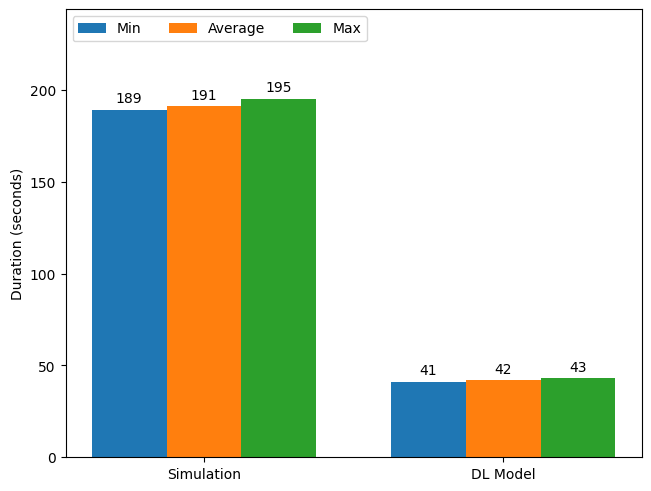
\includegraphics[width=0.7\linewidth]{images/execution_time.png}
%     \caption{Model execution time}
%     \label{fig:ExecutionTime}
% \end{figure}


\begin{table}[ht]
    \caption{CFD simulation vs DL Model execution time}
    \centering
    \begin{tabular}{|c|c|}
    \hline
                    & Average Execution Time \\ \hline
    CFD Simulation  & 191 \\ \hline
    DL Model        & 42 \\ \hline
    \end{tabular}
    \label{tab:ExecutionTime}
\end{table}

